\documentclass[10pt,a4paper]{scrartcl}
\usepackage[utf8x]{inputenc}
\usepackage[english,german]{babel}
\usepackage{amsmath}
\usepackage{amssymb}
\usepackage{graphicx}
\usepackage{listings}
\usepackage[format=plain,indention=1cm,font=sf ,labelfont=bf, nooneline,center]{caption}
\renewcommand{\captionfont}{\sffamily \slshape}
\renewcommand{\captionlabelfont}{ \sffamily \slshape \bfseries   }
\usepackage{subcaption}
\usepackage{url}
\usepackage{empheq}
\usepackage{dcolumn}
\usepackage{rotating}
\newcolumntype{d}{D{.}{.}{-1} }

\usepackage{tikz}
\usetikzlibrary{circuits.ee.IEC,matrix}

% Quelle https://trucastuces.wordpress.com/2012/10/10/boxed-equations-in-latex/
\newlength\dlf  % Define a new measure, dlf
\newcommand\alignedbox[2]{
    % Argument #1 = before & if there were no box (lhs)
        % Argument #2 = after & if there were no box (rhs)
        &  % Alignment sign of the line
        {
            \settowidth\dlf{$\displaystyle #1$}
            % The width of \dlf is the width of the lhs, with a displaystyle font
                \addtolength\dlf{\fboxsep+\fboxrule}
            % Add to it the distance to the box, and the width of the line of the box
                \hspace{-\dlf}
            % Move everything dlf units to the left, so that & #1 #2 is aligned under #1 & #2
                \boxed{#1 #2}
            % Put a box around lhs and rhs
        }
}

\title {Physikalisches Fortgeschrittenenpraktikum I\linebreak
Halbleiterbauelemente}
\author {\emph{Clemens Kurzenberg}\\212204196}
\date {16.04.2015}

\begin{document}

\maketitle

\begin{abstract}
Inhalt des Versuches ist die Analyse von Halbleiterdioden unter Einfluss von
Wechselstrom.
Dazu wird zunächst das Verhalten einer einzelnen Halbleiterdiode untersucht
und anschließend eine Gleichrichterschaltung.
\end{abstract}

\tableofcontents

\pagebreak
\section {Einführung}

Im Versuch untersucht werden eine einzelne Halbleiterdiode und eine
Gleichrichterschaltung.
Die verwendeten Geräte sind in Tabelle \ref{tab:devices} auf Seite
\pageref{tab:devices} verzeichnet.

\subsection {Halbleiterdiode}

Der erste Teilversuch erfolgt mit dem Aufbau in Abbildung \ref{fig:HL_Diode}.

\begin{figure}[!ht]
    \centering
    \begin{tikzpicture}[%show background rectangle,
    circuit ee IEC, circuit symbol lines/.style={draw,thick},
    font=\sffamily\upshape,
    >=latex % Voreinstellung für Pfeilspitzen
    ]
        \matrix (S) [
            matrix of nodes, nodes in empty cells,
            inner sep=0pt, outer sep=-.5\pgflinewidth,
            column sep=20mm, row sep = 7mm,
            nodes={minimum width=0pt}
        ]
        {
            &&&  \\
            &&&  \\
            &&&  \\
        };

        % Bauteile
        \draw (S-1-1)   to [resistor={info=$R_v$, name=R}](S-1-3)
                        to [diode={info=$D$, name=D}](S-3-3);

        % Leiter
        \draw   (S-1-3) -- (S-1-4)
                (S-3-1) -- (S-3-4);

        % Klemmen, Knoten
        \draw [fill=white]  (S-1-1) circle (2pt)
                            (S-1-4) circle (2pt)
                            (S-3-1) circle (2pt)
                            (S-3-4) circle (2pt);

        \draw [fill=black]  (S-1-3) circle (2pt)
                            (S-3-3) circle (2pt);

        \draw   (S-2-1) node {$U_e$}
                (S-2-4) node {$U_a$};
    \end{tikzpicture}
    \caption{Halbleiterdiode im Wechselstromkreis} \label{fig:HL_Diode}
\end{figure}

Das Ersatzschaltbild einer Halbleiterdiode ist in Abbildung \ref{fig:HL_Ersatz}
gezeigt.

\begin{figure}[!ht]
    \begin{subfigure}{\textwidth}
        \centering
        \begin{tikzpicture}[%show background rectangle,
        circuit ee IEC, circuit symbol lines/.style={draw,thick},
        font=\sffamily\upshape,
        >=latex % Voreinstellung für Pfeilspitzen
        ]
            \matrix (S) [
                matrix of nodes, nodes in empty cells,
                inner sep=0pt, outer sep=-.5\pgflinewidth,
                column sep=10mm, row sep = 9mm,
                nodes={minimum width=0pt}
            ]
            {
                &&&&&&&  \\
                &&&&&&&  \\
                &&&&&&&  \\
            };

            % Bauteile
            \draw (S-2-1)   to [inductor={info=$L_1$}] (S-2-3)
                            to [resistor={info=$R_B$, name=RB}](S-2-5)
                            to [resistor={info=$R_D$, name=RD}](S-2-7)
                  (S-1-5)   to [capacitor={info=$C_S$, name=CS}](S-1-7)
                  (S-3-5)   to [capacitor={info=$C_D$, name=CD}](S-3-7);

            % Leiter
            \draw   (S-2-7) -- (S-2-8)
                    (S-1-5) -- (S-3-5)
                    (S-1-7) -- (S-3-7);

            % Klemmen, Knoten
            \draw [fill=white]  (S-2-1) circle (2pt)
                                (S-2-8) circle (2pt);

            \draw [fill=black]  (S-2-5) circle (2pt)
                                (S-2-7) circle (2pt);
        \end{tikzpicture}
        \caption{Durchlassrichtung}
    \end{subfigure}
    \begin{subfigure}{\textwidth}
        \centering
        \begin{tikzpicture}[%show background rectangle,
        circuit ee IEC, circuit symbol lines/.style={draw,thick},
        font=\sffamily\upshape,
        >=latex % Voreinstellung für Pfeilspitzen
        ]
            \matrix (S) [
                matrix of nodes, nodes in empty cells,
                inner sep=0pt, outer sep=-.5\pgflinewidth,
                column sep=10mm, row sep = 9mm,
                nodes={minimum width=0pt}
            ]
            {
                &&&&&&&  \\
                &&&&&&&  \\
            };

            % Bauteile
            \draw (S-2-1)   to [inductor={info=$L_1$}] (S-2-3)
                            to [resistor={info=$R_B$, name=RB}](S-2-5)
                            to [resistor={info=$R_S$, name=RS}](S-2-7)
                  (S-1-5)   to [capacitor={info=$C_S$, name=CS}](S-1-7);

            % Leiter
            \draw   (S-2-7) -- (S-2-8)
                    (S-1-5) -- (S-2-5)
                    (S-1-7) -- (S-2-7);

            % Klemmen, Knoten
            \draw [fill=white]  (S-2-1) circle (2pt)
                                (S-2-8) circle (2pt);

            \draw [fill=black]  (S-2-5) circle (2pt)
                                (S-2-7) circle (2pt);
        \end{tikzpicture}
        \caption{Sperrrichtung}
    \end{subfigure}
    \caption{Ersatzschaltbild einer Halbleiterdiode\\
    $L_1,R_B$ -- Induktivität und Widerstand des Bauelementes\\
    $C_S$ -- Sperrschichtkapazit\\
    $C_D$ -- Diffusionskapazität\\
    $R_D,R_S$ -- Durchlass- und Sperrwiderstand}
    \label{fig:HL_Ersatz}
\end{figure}

Dioden zeichnen sich durch ihre Eigenschaft aus, Strom nur in eine Richtung,
die Durchlassrichtung, zu leiten.
Bei angelegter Rechteckspannung stellt sich beim Umklappen in die Sperrrichtung
eine konstante Sperrkapazität ein, die der in etwa der angelegten Spannung
gleicht.
Dies geschieht nach einer endlichen Zeit, die benötigt wird,
um die Sperrschichtkapazität $C_S$ aufzuladen.
Diese Zeit $t_E$ heißt \emph{Sperrerholzeit}.
Nach dieser Zeit stellt sich zudem ein endlicher \emph{Dunkelstrom} durch
Diffusion von Ladungsträgern in Sperrrichtung ein.
Die \emph{Sperrverzögerungszeit} vom Umklappen der Spannung bis zum
Nulldurchgang $t_s$ wird im Experiment in Abhängigkeit des Durchlass- und
Sperrstroms ermittelt.
In dieser Zeit ist der Sperrstrom konstant.

\subsection {Gleichrichterschaltung}

Die Gleichrichterschaltung wird nach Abbildung \ref{fig:Gleichrichter}
aufgebaut.

\begin{figure}[!ht]
    \centering
    \begin{tikzpicture}[%show background rectangle,
    circuit ee IEC, circuit symbol lines/.style={draw,thick},
    font=\sffamily\upshape,
    >=latex % Voreinstellung für Pfeilspitzen
    ]
        \matrix (S) [
            matrix of nodes, nodes in empty cells,
            inner sep=0pt, outer sep=-.5\pgflinewidth,
            column sep=10mm, row sep = 7mm,
            nodes={minimum width=0pt}
        ]
        {
            &&&&&&&&&  \\
            &&&&&&&&&  \\
            &&&&&&&&&  \\
            &&&&&&&&&  \\
            &&&&&&&&&  \\
        };

        \tikzset{
            Pfeil/.style={thick,shorten >=#1,shorten <=#1,->}, % für Peile
            UPfeil/.style={blue,Pfeil=#1,font={\sffamily\itshape}},% für Spannungspfeile
            IPfeil/.style={red,Pfeil=#1,font={\ttfamily\itshape}} % für Strompfeile
        }


        % Bauteile
        \draw (S-1-2)   to [diode={name=D1}](S-1-4) to (S-1-6)
                        to [resistor={info=$R_{39}$, name=R1}](S-1-8)
                        to [resistor={info=$R_{39'}$, name=R2}](S-3-8)
                        to [capacitor={info=$C_1$, name=C1}](S-5-8)
              (S-2-6)   to [capacitor={info=$C_2$, name=C2}](S-4-6)
              (S-2-9)   to [resistor={info=$R_L$, name=C2}](S-4-9)
              (S-2-4)   to [diode={name=D2}](S-2-2)
              (S-4-2)   to [diode={name=D3}](S-4-4)
              (S-5-4)   to [diode={name=D4}](S-5-2);

        % Leiter
        \draw   (S-1-8) -- (S-1-10)
                (S-5-4) -- (S-5-10)
                (S-1-9) -- (S-2-9)
                (S-4-9) -- (S-5-9)
                (S-1-6) -- (S-2-6)
                (S-4-6) -- (S-5-6)
                (S-1-2) -- (S-2-2)
                (S-4-2) -- (S-5-2)
                (S-2-1) -- (S-2-2)
                (S-4-1) -- (S-4-2)
                (S-5-4) -- (S-2-4)
                (S-4-4) -- (S-4-5) -- (S-1-5);

        % % Klemmen, Knoten
        \draw [fill=white]  (S-2-1) circle (2pt)
                            (S-1-10) circle (2pt)
                            (S-4-1) circle (2pt)
                            (S-5-10) circle (2pt);

        \draw [fill=black]  (S-1-9) circle (2pt)
                            (S-5-9) circle (2pt)
                            (S-1-8) circle (2pt)
                            (S-5-8) circle (2pt)
                            (S-1-6) circle (2pt)
                            (S-5-6) circle (2pt)
                            (S-2-2) circle (2pt)
                            (S-4-2) circle (2pt)
                            (S-5-4) circle (2pt)
                            (S-1-5) circle (2pt);

        \draw   (S-3-1) node {$U_e$}
                (S-3-10) node {$U_a$};

        \draw[UPfeil=0.25em] ([yshift=4mm]S-1-2.north) --
        ([yshift=4mm]S-1-3.north) node[midway, above]{$U^+$};
        \draw[UPfeil=0.25em] ([yshift=-4mm]S-5-4.north) --
        ([yshift=-4mm]S-5-3.north) node[midway, anchor=north]{$U^+$};
        \draw[UPfeil=0.25em] ([yshift=4mm]S-4-2.north) --
        ([yshift=4mm]S-4-3.north) node[midway, above]{$U^-$};
        \draw[UPfeil=0.25em] ([yshift=-4mm]S-2-4.north) --
        ([yshift=-4mm]S-2-3.north) node[midway, anchor=north]{$U^-$};
    \end{tikzpicture}
    \caption{Gleichrichterschaltung\\
    Verlauf unterschiedlicher Stromrichtungen durch Pfeile mit $U^\pm$ angegeben}
    \label{fig:Gleichrichter}
\end{figure}

$U_e$ ist hierbei gegeben durch einen massenfreien Transformator.
$C_1$, $C_2$ und $R_{39'}$ sind im Verlauf des Versuches an einigen Stellen
entfernt, was durch $C=0$ oder $R=0$ angegeben wird.

Diese Schaltung soll dazu dienen, aus einem Wechselstromsignal ein möglichst
gutes Gleichstromsignal zu machen.
Die vier Dioden sorgen dafür, dass der Strom im restlichen Kreis nur in eine
Richtung fließen kann.

Wenn $C_2=0$ ist, dann ist $C_1$ ein sogenannter \emph{Ladekondensator},
der das Signal durch eine dem Strom entgegengesetzte Spannung erstmal abflacht.
Die entstehende Spannung beinhaltet immer noch Oszillationen und wird
\emph{Brummspannung} genannt.
In diesem Fall übernimmt $R_{39}$ nur die Rolle eines Messwiderstandes.

Ist $C_2\not0$, übernimmt dieser die Rolle des Ladekondensators
und $C_1$ bildet mit $R_{39}$ einen Tiefpass, der das Signal weiter abflacht.
Dieser Tiefpass wird \emph{Siebglied} genannt.
as übrig bleiben sollte, ist eine gute Näherung an Gleichstrom.

Zur Untersuchung des Signals wird der \emph{Stromflusswinkel} betrachtet.
Er beschreibt das Verhältnis der Zeit $t_1$,
in der ein Signal übertragen wird gegenüber der gesamten Periodendauer $T$,
projiziert auf einen Vollwinkel.

\begin{equation}
    \Phi\,=\,\frac{t}{T}\,360^\circ
\end{equation}

\section {Durchführung}

\subsection {Halbleiterdiode}

Als Vorwiderstand wird $R_v=10~\mathrm{k\Omega}$ gewählt.
Der Strom wird durch einen Funktionsgenerator als Rechteckspannung der
Frequenz $\nu=2.194\mathrm{kHz}$ geliefert.

Im Folgenden wird mit $U_e$ die eingehende Spannung, mit $U_{p-p}$ deren
Peak-to-Peak-Wert, mit $U_o$ der Betrag über $0~\mathrm V$ und $U_u$ der
Betrag unter $0~\mathrm V$ bezeichnet.
$U_a$ ist die ausgehende Spannung, $U_R$ die, die am Widerstand abfällt,
$U_D$ die Durchlassspannung an der Diode und $U_S=U_u$ deren Sperrspannung.
Analog sind $I_D$ und $I_S$ Durchlass- und Sperrstrom der Diode.

Gemessen werden jeweils $U_{p-p}$, $U_D$ und $t_s$.
Zunächst wird $U_o=1.51~\mathrm V$ konstant gehalten und $U_{p-p}$ variiert.
Dadurch ändert sich $U_u=U_S$ und für den Strom gilt
$I_S=\frac{U_S}{R_v}=\frac{U_{p-2}-U_o}{R_v}$.
Anschließend wird $U_u=1.49~\mathrm V$ konstantgehalten, $U_{p-p}$ und
analog $I_D=\frac{U_o-U_D}{R_v}=\frac{U_{p-2}-U_u-U_D}{R_v}$ berechnet.

% TODO: Wertetabellen

Die Ergebnisse sind in Abbildung \ref{fig:HL_t_s} dargestellt.

\begin{figure}[!ht]
    \begin{subfigure}{\textwidth}
        \centering
        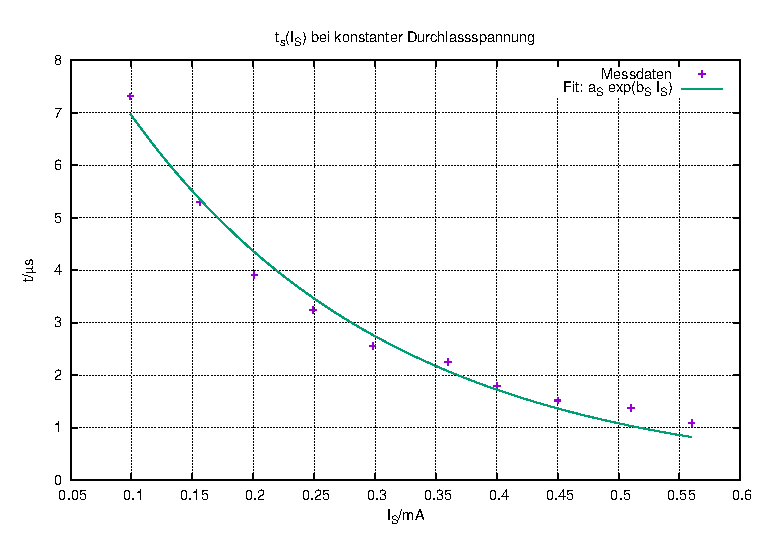
\includegraphics[width=0.7\textwidth]{graphics/diode_I_t_durchlass.eps}
        \caption{$t_s(I_S)$ bei $I_D=\text{const}$}
    \end{subfigure}
    \begin{subfigure}{\textwidth}
        \centering
        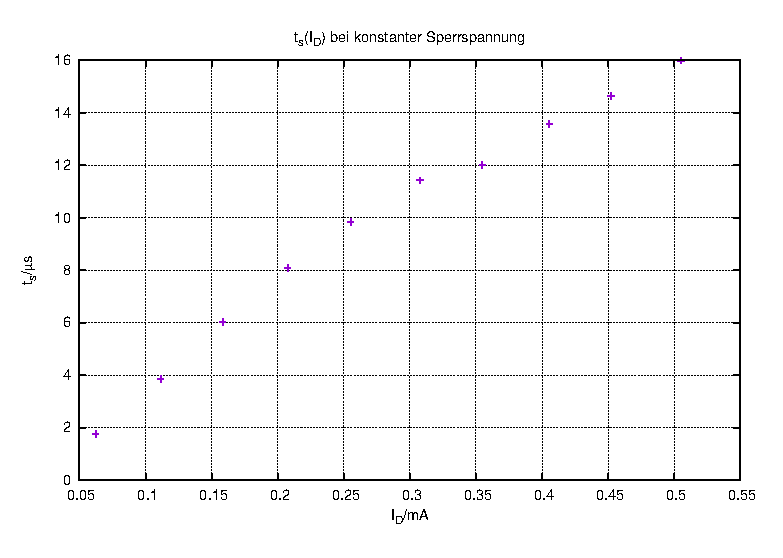
\includegraphics[width=0.7\textwidth]{graphics/diode_I_t_sperr.eps}
        \caption{$t_s(I_D)$ bei $I_S=\text{const}$}
    \end{subfigure}
    \caption{Verhalten von $t_s$ in Abhängigkeit von Sperrstrom $I_S$ und
    Duchlassstrom $I_D$}
    \label{fig:HL_t_s}
\end{figure}

\subsection {Gleichrichterschaltung}

Für die massenfreien Spannungsversorgung wird ein Transformator von Netzspannung
$220~\mathrm V/50~\mathrm{Hz}$ auf $6~\mathrm V/50~\mathrm{Hz}$ verwendet.
Der Lastwiderstand beträgt $R_L=10~\mathrm{k\Omega}$.

Zunächst sei $C_2=0$ und $R_{39}=R_{39}'=39~\Omega$.
Gemessen werden die Spannungen über die Messwiderstände $R_{39}$, $R_{39}'$
und den Lastwiderstand $R_L$,
namentlich $U_R$, $U_C$ und $U_a$.
Das Signal $U_C$ wird invertiert, da man an dieser Stelle gegen den Strom misst.
Aus diesem Messgrößen lassen sich die Ströme über Dioden, Kondensator und
Signalausgang berechnen.

\begin{align}
    I_D \,&=\,\frac{U_R}{R_{39}}\\
    I_C \,&=\,\frac{U_C}{R_{39}'}\\
    I_a \,&=\,\frac{U_a}{R_L}
\end{align}

Für $C_1=0$ und $C_1=10~\mathrm{\mu F}$ sind die Spannungssignale in Abbildung
\ref{fig:Gleichrichter_U} und die Ströme in Abbildung
\ref{fig:Gleichrichter_I} ab Seite \pageref{fig:Gleichrichter_U} dargestellt.

\begin{figure}[!ht]
    \begin{subfigure}{\textwidth}
        \centering
        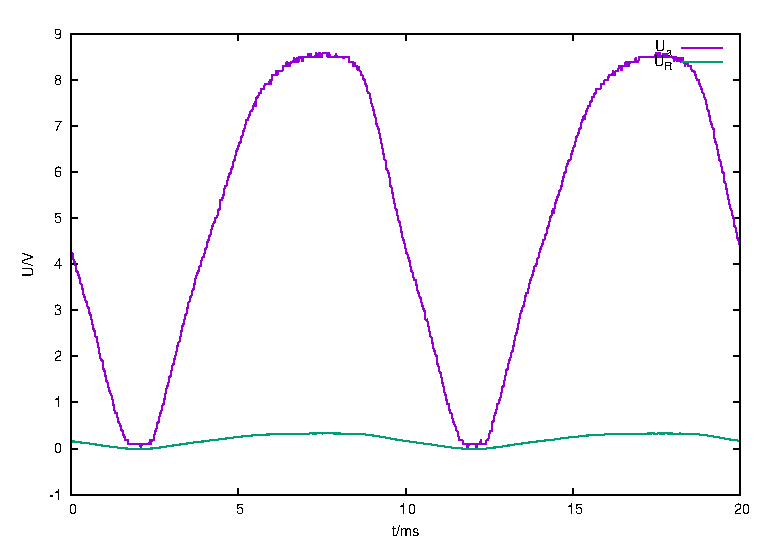
\includegraphics[width=0.7\textwidth]{graphics/gleichrichter_0F.eps}
        \caption{$C_1=0$}
    \end{subfigure}
    \begin{subfigure}{\textwidth}
        \centering
        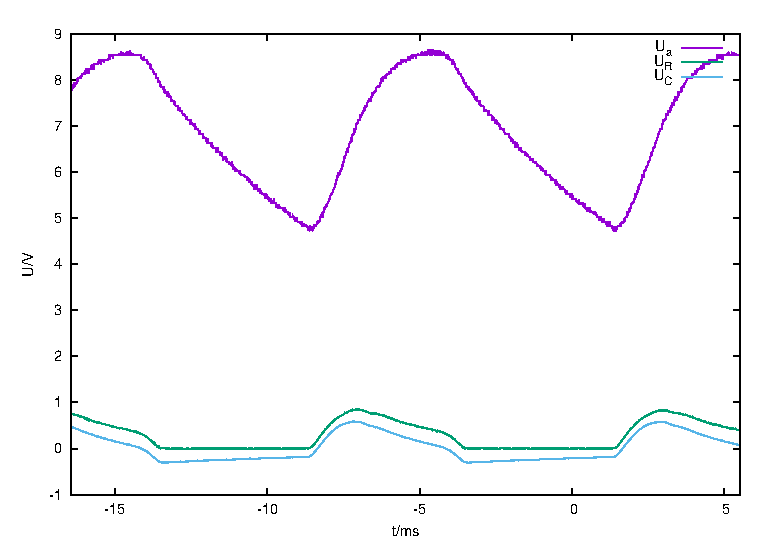
\includegraphics[width=0.7\textwidth]{graphics/gleichrichter_10uF.eps}
        \caption{$C_1=10~\mathrm{\mu F}$}
    \end{subfigure}
    \caption{Spannungen im Gleichrichter mit $C_2=0$ und $R_{39}'=R_{39}$ für
        die Fälle $C_1=0$ und $C_1=10~\mathrm{\mu F}$}
    \label{fig:Gleichrichter_U}
\end{figure}

\begin{figure}[!ht]
    \begin{subfigure}{\textwidth}
        \centering
        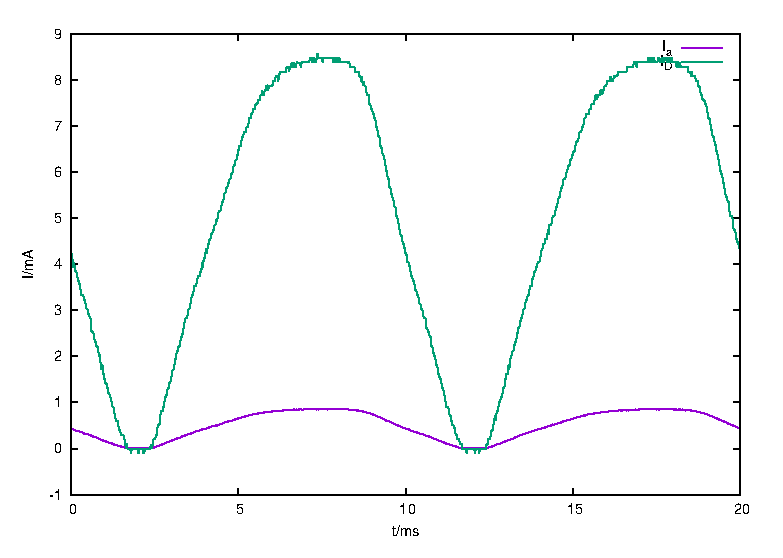
\includegraphics[width=0.7\textwidth]
            {graphics/gleichrichter_strom_0F.eps}
        \caption{$C_1=0$}
    \end{subfigure}
    \begin{subfigure}{\textwidth}
        \centering
        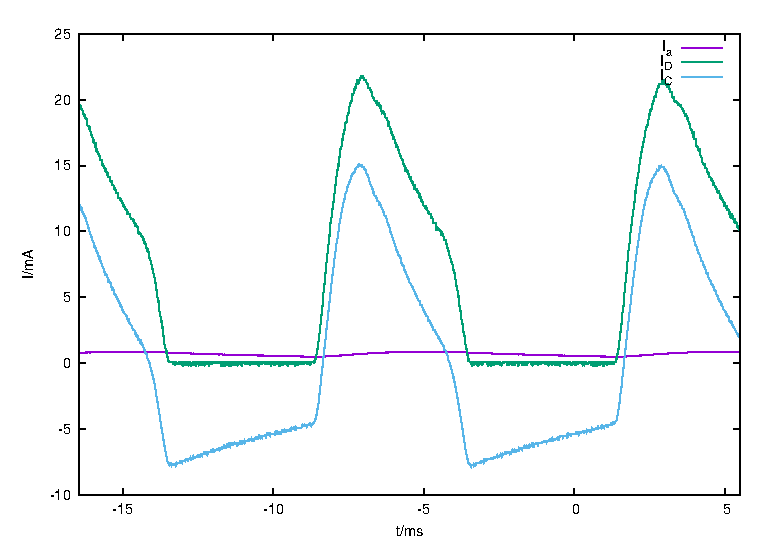
\includegraphics[width=0.7\textwidth]
            {graphics/gleichrichter_strom_10uF.eps}
        \caption{$C_1=10~\mathrm{\mu F}$}
    \end{subfigure}
    \caption{Ströme im Gleichrichter mit $C_2=0$ und $R_{39}'=R_{39}$ für
        die Fälle $C_1=0$ und $C_1=10~\mathrm{\mu F}$}
    \label{fig:Gleichrichter_I}
\end{figure}

Für $C_1=0$ ist das Signal an Widerstand $C_{39}$ und Ausgang zu gleichen Zeiten
der Länge $t_{0,0}=608~\mathrm{ns}$ null.
Aufgrund der angelegten $50~\mathrm{Hz}$ ist $T=10~\mathrm{ms}$.
Damit ist der Stromwinkel hier $\Phi_0=338^\circ$.

Für $C_1=10~\mathrm{\mu F}$ ist $U_a$ nie null,
sodass $\Phi_{10~\mathrm{\mu F},a}=360^\circ$ ist.
Am Widerstand ist das Signal jedoch für eine Dauer
$t_{10~\mathrm{\mu F},0}=4.84~\mathrm{ms}$ null.
An den Dioden ist der Stromwinkel also
$\Phi_{10~\mathrm{\mu F},D}=185.76^\circ$.

Um zu sehen, wie gut der Gleichrichter funktioniert,
wird die Ausgangsspannung $U_a$ für verschiedene Fälle aufgenommen,
in denen $R_{39}'=0$ ist.
Der Vergleich ist in Tabelle \ref{tb:Gleichrichter} auf Seite
\pageref{tb:Gleichrichter} protokolliert.
Die Spannungsverläufe sind in Abbildung \ref{fig:Gleichrichter_U2} aufgetragen.

\begin{table}[!ht]
    \centering
    \caption{Vergleich der Gleichrichterschaltung für verschiedene Parameter
    mit $R_{39}'=0$}
    \label{tb:Gleichrichter}
    \begin{tabular}{r|r|l|l|l}
        $C_1/\mathrm{\mu F}$&$C_2/\mathrm{\mu F}$&$U_{p-p}/\mathrm V$
        &$U_{avg}/\mathrm V$&$U_{top}/\mathrm V$\\
        \hline
        0&0&8.8&5.15&8.8\\
        10&0&3.9&6.68&8.3\\
        100&0&0.70&6.51&7.7\\
        100&100&0.23&8.06&8.15\\
    \end{tabular}
\end{table}

\begin{figure}
    \centering
    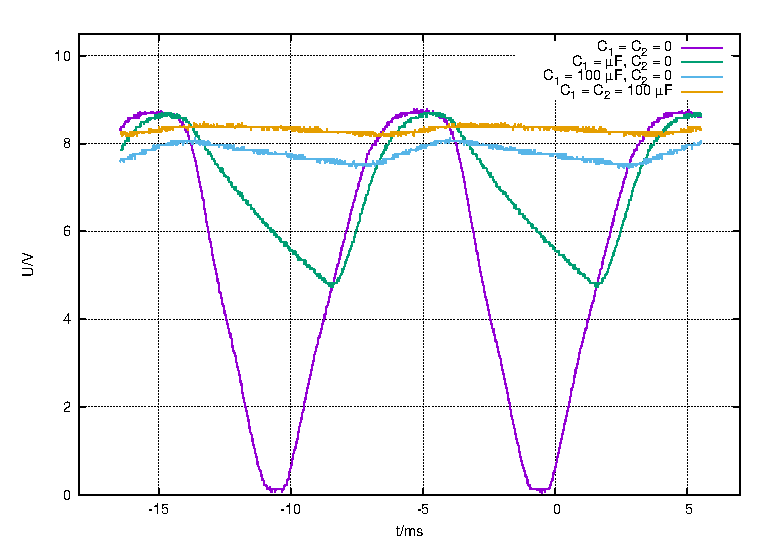
\includegraphics[width=\textwidth]{graphics/gleichrichter_spannungen.eps}
    \caption{Spannungsverläufe $U_a$ im Gleichrichter für unterschiedliche
    $C_1$ und $C_2$}
    \label{fig:Gleichrichter_U2}
\end{figure}


\section {Auswertung}

% TODO

% \pagebreak
% \section {Quellen}
% \begin{thebibliography}{999}
% \bibitem {WalterHerms} G. Walter und G. Herms, Einführung in die Behandlung von Messfehlern -- Ein Leitfaden für das Praktikum der Physik, Universität Rostock 2006d
% \end{thebibliography}

\section {Anhang}

\begin{table}[ht!]
    \centering
    \caption{verwendete Geräte} \label{tab:devices}
    \begin{tabular}{lr}
        Arbeitsplatz & 9\\
        Oszilloskop&Agilent Technologies Infiicision MSO-X 2002A\\
        Funktionsgenerator&FG1617 Function Generator\\
        Mini $\Omega$ Dekade&RT 1-1000 SAB\\
        Steckbrett & 4
    \end{tabular}
\end{table}


\end{document}
%sagemathcloud={"zoom_width":100}
